\chapter{Zusammenfassung und Ausblick}
In diesem Projekt handelt es sich um eine Anwendung, die au�ergew�hnliche Situationen erkennen kann. Die Applikation orientiert sich an alten Menschen, die allein wohnen. Das Projekt ist eine Kombination von Hintergrundsubtraktion, Histogrammanalyse und Wahrscheinlichkeitsanalyse. Auf diesen Ziel und Verfahren macht dieses Projekt so besonders und zugleich interessant. Das hat mich dazu motiviert, dieses Projekt zu entwickeln. \\

Ziel dieses Projekt ist die Entwicklung eine Anwendung, das mit Videos von einer Bosch-360-Grad-Kamera verarbeitet. Das Programm soll eine Bewegung von einer Person erkennen, analysiert und Informationen geben, ob die Person in einer au�ergew�hnlichen Situation stattfindet. Eine abnormale Situation handelt sich um Liegen von der Person auf dem nicht normalen Ort und die Person kann  in einem bestimmten Zeitraum sich nicht bewegen. Um dieses Ziel zu realisieren, wurde das Programm aus drei gro�en Meilensteinen gebaut (Abbildung \ref{fig:zusammenfassung}). Der erste Meilenstein ist die Hintergrundsubtraktion. In diesem Schritt wird ein Bild als eine Eingabe mit einem Hintergrundbild vergleichen. Der Unterschied zwischen des Eingabebildes und Hintergrundbildes wird zuerst berechnet und ein Bin�rbild von dem Vordergrund wird danach zur�ckgeliefert. Eine Region der Bewegung wird mithilfe einer Begrenzungsbox beschr�nkt. Diese beschr�nkte Region wird in dem n�chsten Schritt ganz n�tzlich. Das Hintergrundbild wird immer nach Eingabe eines Bildes aktualisiert, wobei die  beschr�nkte Region nicht mit aktualisiert wird. Das hilft der Person immer gut von dem Hintergrund segmentiert, obwohl die Person nicht mehr in der Szene sich nicht bewegt. In dem zweiten Schritt wird die beschr�nkte Silhouette vom dem letzten Schritt weiter analysiert, um die K�rperhaltung der Person zu erkennen. Die Silhouette wird zuerst von der Breite oder H�he auf 128 Pixel skaliert. Aus dem skalierten Bild werden vertikale und horizontale Histogramme gerechnet. Die Histogramme wird weiter mit die vordefinierte normalisierte vertikale und horizontale Histogramme, die aus 4500 Silhouetten von 7 verschiedenen Personen mit 4 K�rperhaltungen (Liegen, Stehen, Beugen, Sitzen), verglichen. Nach dem Vergleichen wird die K�rperhaltung mit  einem maximalen Wert von Loglikelihood-Funktion ausgefiltert. In letztem Schritt wird eine Fuzzymodell angewendet. Das Modell berechnet einfach wie hoch die Wahrscheinlichkeit, dass eine Person unter bestimmten Bedingungen in eine abnormale Situation, ist. Die Bedingung, die f�r einen abnormalen Fall erf�llt werden m�ssen, ist, wenn eine Person  auf dem Boden in einem vordefinierten Zeitraum (f�r Testen sind 30 Bildern aber das Parameter kann f�r spezielle F�lle modifiziert werden) liegt und sich nicht mehr bewegt. Ein vorgesungenes Feature  von der Bosch-360-Grad Kamera ist die F�higkeit, in die Richtigen der Bewegung zu orientieren. Das wird auch in diesem Projekt mitgebracht und liefert Ergebnisse wie die Erwartungen zur�ck.\\
\begin{figure}[H]
	\centering
	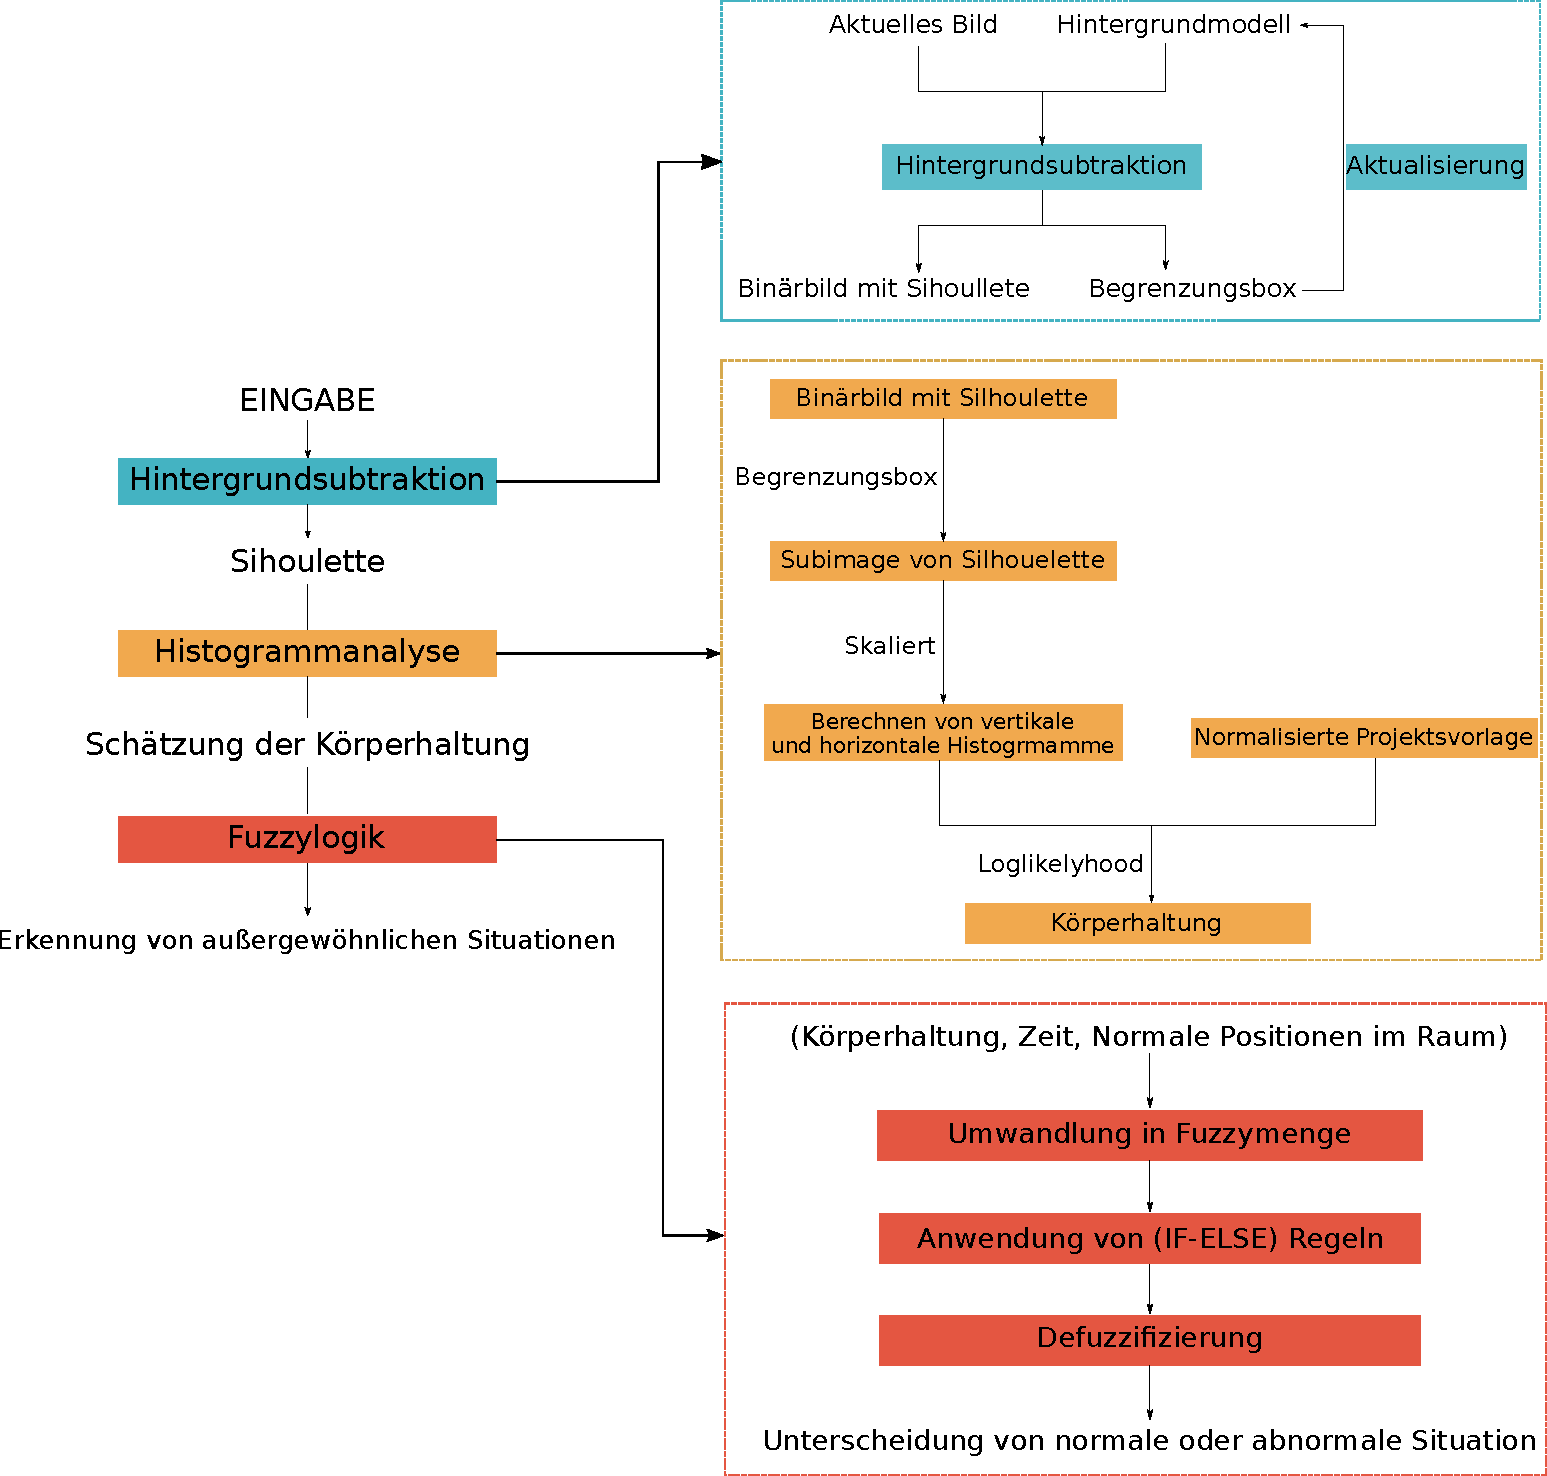
\includegraphics[width=1\textwidth]{fig/zusammenfassung.pdf}
	\caption{Zusammenfassung des Programmaufbaus} 
	\label{fig:zusammenfassung}
\end{figure}
 Um die Ergebnisse von dem Projekt zu evaluieren, wird jedes Testvideos w�hrend der Teste notiert. Die Testergebnisse wurden mit unseren erwartetet Werte verglichen. Das Programm kann alle au�ergew�hnlichen Situationen richtig erkennen und die K�rperhaltung der Person genau sch�tzen. Die Herausforderung der Arbeit besteht darin, die Verarbeitungszeit m�glichst gering zu halten. Bei einer durchschnittlichen Rechnerzeit von 109 Millisekunden pro Frame kann das Projekt als eine Echtzeitanwendung benutzt werden.\\
 
 Das Projekt hat viele Erweiterungspotenziale. Mir sind noch ein paar Ideen eingefallen, um das Programm noch umfangreicher zu machen.  Die erste Idee basiert auf der F�higkeit der Bewegungserkennung des Projektes. Die Kamera kann als einen Abwesenheitsmelder angewendet. Wenn es keine Bewegung in Haus in 24 Stunden gibt, dann wird ein Abwesenheitsmelder ausgel�st oder ein Sicherheitsalarm wird automatisch angeschaltet. Zweite Idee ist eine Erweiterung des Projektes. Bis jetzt die Kamera wird noch nicht mit der Smart Home App integriert. Wenn die M�glichkeit Integrieren der Kamera mit der App realisiert werden kann, wird eine automatisch Lichtschalter oder Heizungsschalter sofort nach Erkennung einer Bewegung aktiviert. Die dritte Idee ist eine Verbesserung des Projektes. Heutzutage wird k�nstliche Intelligenz �berall verwendet. Mit Hilfe von neuronale Netz mit riesigem Datens�tzen kann die Sch�tzung der K�rperhaltung verbessert werden und damit wird auch die Qualit�t der Software auch deutlich erh�ht.